\chapter{Systematic Uncertainties}
The signal and background processes are affected by a variety of systematic effects that contribute to an overall uncertainty in the yields of each. Understanding these systematic uncertainties is important not only for undertaking a statistical analysis of the results, but also to ensure that no systematic is overly constrained when they are fit during the limit calculation.

The largest systematic uncertainty impacting this search is the uncertainty in the jet mass scale and resolution. By comparing the jet mass resolution using the \textsc{Delphes} framework to the resolution in Run 2, as is done in \cref{fig:jmr}, it is apparent that the former is likely overly optimistic of the eventual Phase-2 resolution. To account for the uncertainty in the eventual resolution and scale, the AK8 jet mass distribution is smeared and shifted by a Gaussian distribution, which is good approximation for the Run 2 resolution near $m_\mathrm{h}$. This new distribution is then used to calculate signal region yields which are compared to the original yields to obtain a nuisance as shown in \cref{eq:nuis}.

\begin{figure}[ht]
\centering
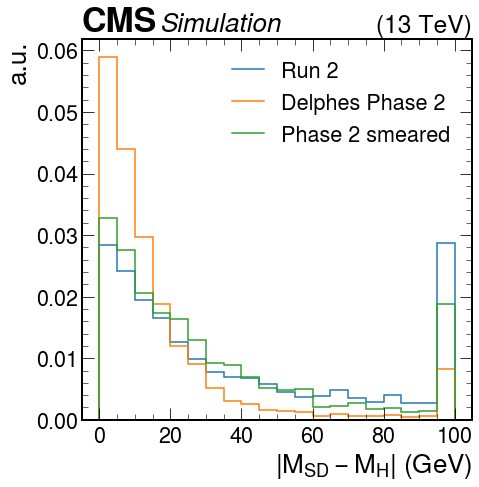
\includegraphics[width=0.6\textwidth]{Chapters/Systematics/jmr.png}
\caption{The absolute difference between the AK8 jet soft drop mass and $m_\mathrm{h}$. Plotted are t$\bar{\mathrm{t}}$h samples from Run 2, \textsc{Delphes}, and \textsc{Delphes} with the Gaussian smearing applied.}
\label{fig:jmr}
\end{figure}

\begin{equation}
    \text{nuisance}_{\pm} = 1\pm\frac{\text{new yield}-\text{old yield}}{\text{old yield}}
    \label{eq:nuis}
\end{equation}

The jet resolution and scale uncertainties are large, but do not employ a more complicated correlation scheme that would likely be used at the HL-LHC. In order to not overly constrain the large uncertainty, flat, partially correlated uncertainties on the mass and \mt binning are assigned. This is done by having an uncertainty correlated in the mass bins, but uncorrelated in the \mt bins and having an uncertainty correlated in the \mt bins, but uncorrelated in the mass bins.

The next largest group of systematic uncertainties come from the theoretical uncertainties affecting the cross-sections of the signals and backgrounds. Uncertainties in the values of $\alpha_S$ are calculated by varying the value of $\alpha_S$ in the simulated events, then comparing the new yields after those variations to the previous yields, similar to the \cref{eq:nuis}. Additional systematic uncertainties come from varying the choice of PDF as well as the factorization scale $\mu_F$ and the renormalization scale $\mu_R$ of the PDF~\cite{Buckley_2015}.

The next largest group of systematic uncertainties comes from uncertainties on the tagging and mistagging rate of the h $\to$ b$\bar{\mathrm{b}}$ tagger. The tag and mistag rates are varied up and down by 10\%. The nuisances are then calculated by taking the difference between the yields when the rates are varied up and down and dividing by the central yields.

The next most prominent systematic uncertainty is the jet energy scale. The uncertainty due to this systematic factor is calculated similarly to the jet mass scale. The jet energies are varied by corrections to the jet energy scale. These corrections are propagated to the \ptmiss. The nuisances are then calculated by taking the difference between the yields when the energies are varied up and down and dividing by the central yields.

Finally, a flat systematic uncertainty of 1\% has been assigned as the uncertainty of the integrated luminosity according to the prescription in~\cite{CMS-PAS-FTR-16-002}. A summary of the systematic uncertainties is given in \cref{tab:systematics}. 

The effects of the small size of the events in the \textsc{Delphes} samples have not been included in this search. However, to avoid an overly aggressive assumption of the uncertainty in the yields, a statistical uncertainty is assigned by taking the square root of the yields for each process in each bin.

\begin{table}
    \center
    \caption{Summary of the effect of the systematic uncertainties used in this analysis on the yields.}
    \begin{adjustbox}{width=\textwidth}
    \begin{tabular}{|l|c|c|c|c|c|c|}
    \hline
	Systematic Uncertainty    & Signal    & t$\bar{\mathrm{t}}$/single-t & W+jets  & Multijet & Z+jets  & SM Higgs   \\ \hline
	Luminosity                & 1\%       & 1\%             & 1\%      & 1\%      & 1\%      & 1\%      \\
	Inclusive cross-section   & -        & 25\%            & -       & 50\%     & -       & -       \\
    JES                       & $<10\%$   & $<10\%$         & $<10\%$  & $<15\%$  & $<11\%$  & $<7\%$   \\
    JMS/JMR                   & $<11\%$   & $<15\%$         & $<10\%$  & $<39\%$  & $<9\%$   & $<25\%$  \\
	JMR mass-uncorrelated       & 6\%       & 6\%             & 6\%      & 6\%      & 6\%      & 6\%      \\
	JMR \mt-uncorrelated        & 4--8\%   & 4--8\%         & 4--8\%  & 4--8\%  & 4--8\%  & 4--8\%  \\
	Higgs tagging               & 10\%      & -             & -       & -      & -       & 10\%     \\
	Higgs mistagging            & $<1\%$    & $<10\%$         & $<10\%$  & $<10\%$  & $<7\%$   & $<1\%$   \\
	PDF			            & 1--6\%   & -              & 1\%-6\%  & -       & 1--18\% & 2--21\% \\
	$\alpha_{\text{S}}$                & $<4\%$    & -              & 1--8\%  & -       & 2--9\%  & $<2\%$   \\
	$\mu_{\text{F}}$ and $\mu_{\text{R}}$       & 21--37\% & -              & 9--22\% & -       & 9--23\% & $<32\%$  \\
	\hline
    \end{tabular}
    \end{adjustbox}
    \label{tab:systematics}
\end{table}


Initially, the main source of uncertainty in each bin comes from the systematic uncertainties, with the jet mass resolution and scale uncertainty contributing the largest amount. However, the systematic uncertainties become constrained during the fit. This can be seen in \cref{fig:srbins}, where after fitting the main source of uncertainty appears to be the statistical uncertainty because it grows in relative strength as the number of events in the bin decreases. As a result, \cref{fig:impacts} shows that the uncertainty in jet mass scale and resolution becomes quite constrained, with some other initially large uncertainties such as the uncertainty in choice of PDF and the multijet production cross-section also being somewhat constrained. This is to be expected, considering that I am partially binning in jet mass and because the uncertainty was so large to begin with.

\begin{figure}[ht]
    \centering
    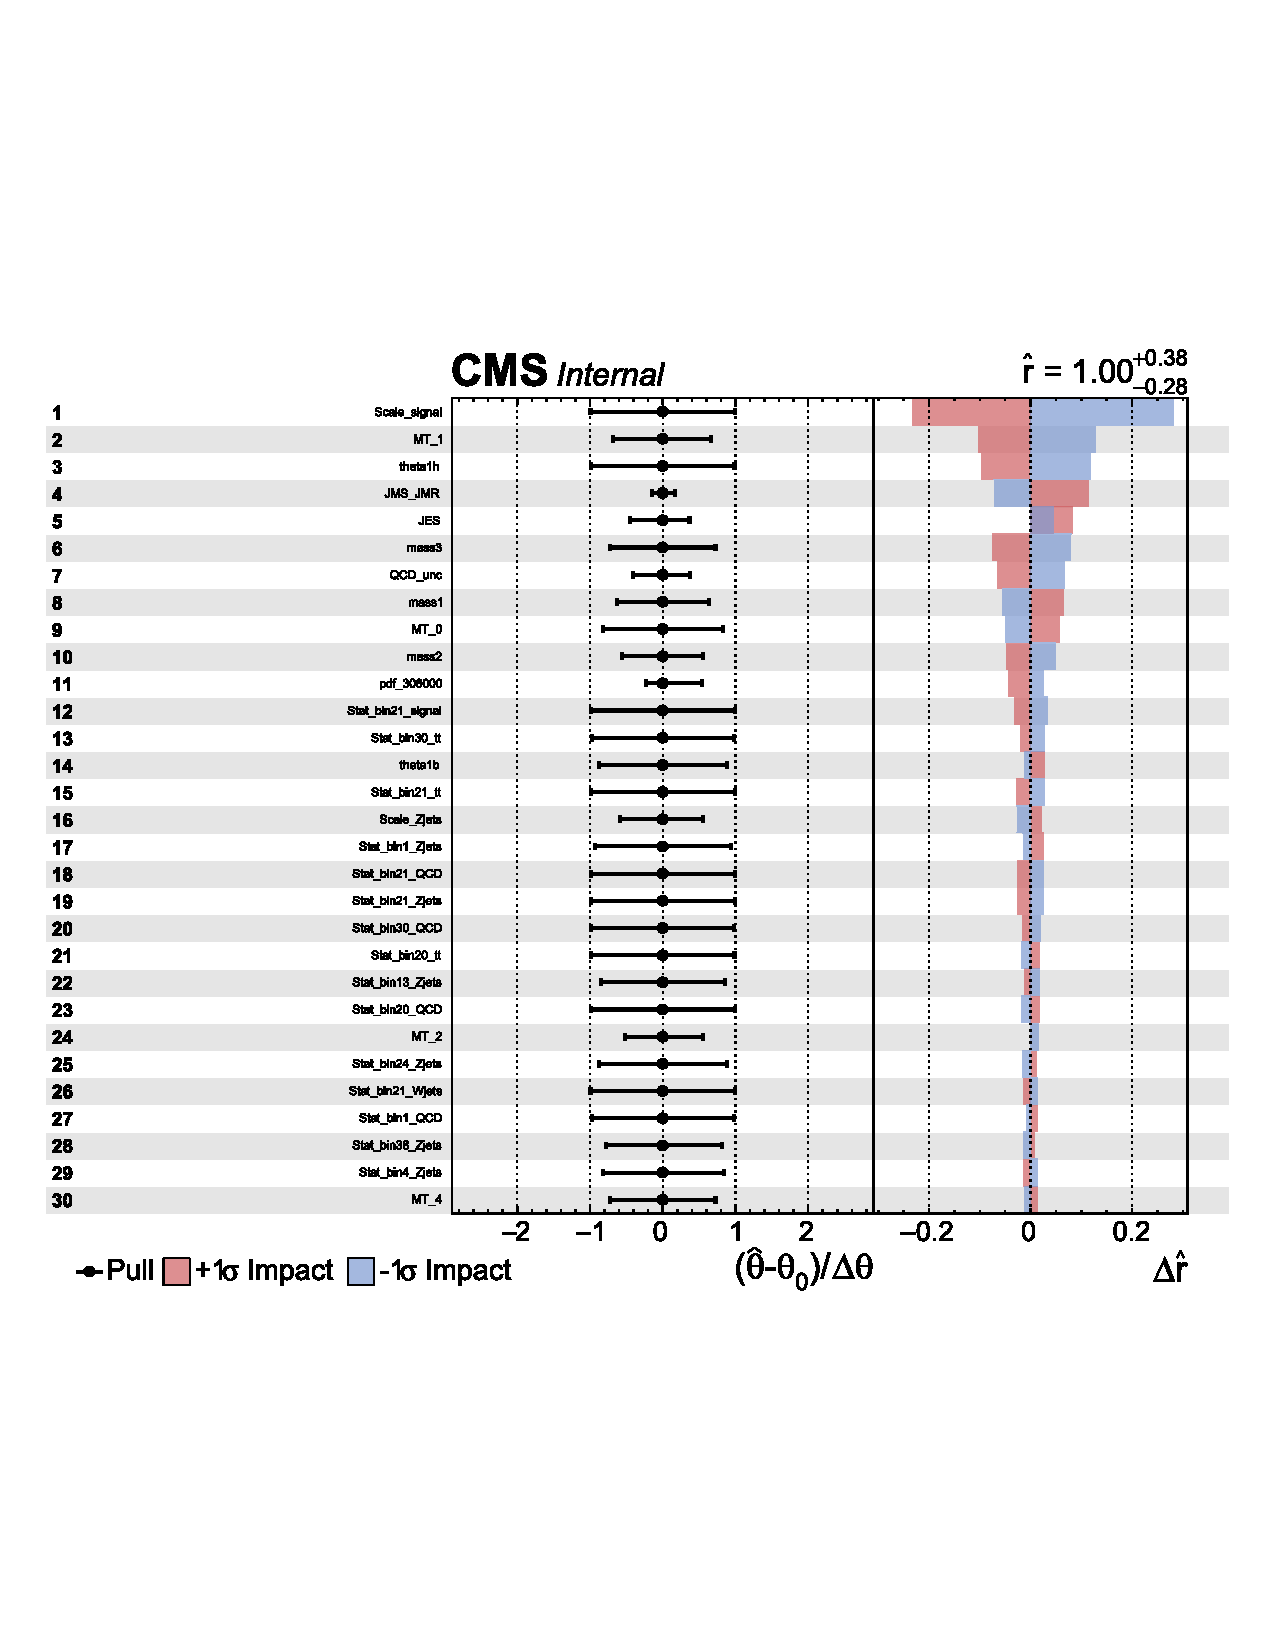
\includegraphics[width=0.9\textwidth]{Chapters/Systematics/impacts_both_sidebands_pg1.pdf}
    \caption{The impacts and pulls of the uncertainties in this search.}
    \label{fig:impacts}
\end{figure}